\documentclass{ximera}
\input{../preamble.tex}

\author{D. Davis \and R. Speckert \and N. Shay \and A. Davis}
\title{Need Title} \license{CC BY-NC-SA 4.0}
\begin{document}

\begin{abstract}
\end{abstract}
\maketitle

\begin{onlineOnly}
\section*{Need Title}
\end{onlineOnly}

\subsection*{Data Collection Activity}

Our best customer placed an order for 100 units of product.  The product is rectangular sheets of silicon that will be sent through a stamping operation to create round wafers. These silicon wafers will be used to manufacture integrated circuit chips. The silicon sheets will be $6.98$cm by $10.79$cm ($2.75$in $\times$ $4.25$in) with a nominal diagonal dimension of $12.85$cm ($5.06$in).  To properly align in the stamping machine, the diagonal specifications must be $12.85$cm $\pm$ $0.15$cm  ($5.06$in $\pm$ $0.06$in).

\begin{question}\label{quest:qc150_1}
What are the upper and lower specification limits in cm and inches for the diagonal dimension?

Upper Specification Limit (USL) $=\answer{13}\text{cm}=\answer{5.12}\text{in}$

Lower Specification Limit (LSL) $=\answer{12.7}\text{cm}=\answer{5}\text{in}$

\end{question}

Supplies needed:
\begin{itemize}
\item 13 sheets of standard copier paper 21.59cm $\times$ 27.94cm (8.5in $\times$ 11in). The paper will be used in place of silicon sheets.
\item 30.48cm (12-inch) ruler. Note that measurements will be recorded in cm.  \href{http://www.vendian.org/mncharity/dir3/paper_rulers/}{Here is a printable ruler.}  Select the first ruler in the list.
\item A computer to enter data into a spreadsheet.
\end{itemize}
Procedure:
\begin{enumerate}
\item	Organize your group (3 students per group) to fulfill the customer's request.   The roles to be played in your group are:
    \begin{itemize}
\item A paper-folder and tearer
\item A measurer
\item A data recorder 
\item All students will serve as statistical analysts.
    \end{itemize}
\item Follow the instructions for folding and tearing the paper in the diagram below.

\begin{center}
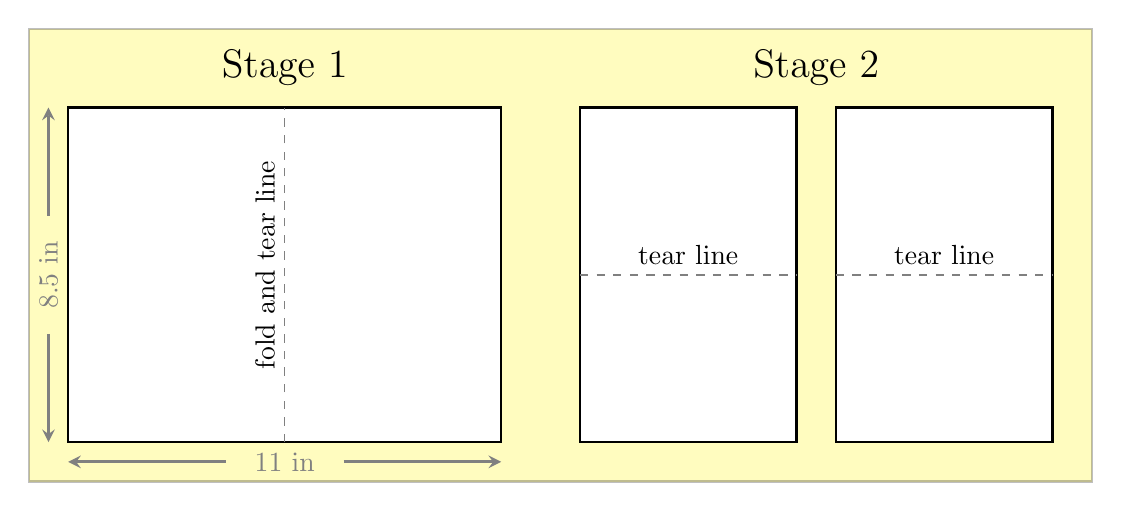
\begin{tikzpicture}[scale=0.5]
\draw[black, thick, fill=yellow,opacity=0.25] (-1,-1) rectangle (26, 10.5);
 \draw[black, thick, fill=white] (0,0) rectangle (11,8.5);
 \draw[line width=0.5pt, dashed, gray](5.5,0)--(5.5,8.5);
\node[rotate=90] at (5,4.5)   {fold and tear line};
\draw[line width=1pt,gray, stealth-](0,-0.5)--(4,-0.5);
\draw[line width=1pt,gray, -stealth](7,-0.5)--(11,-0.5);
\node[gray] at (5.5,-0.5)   {11 in};
\draw[line width=1pt,gray, -stealth](-0.5,2.75)--(-0.5,0);
\draw[line width=1pt,gray, -stealth](-0.5, 5.75)--(-0.5, 8.5);
\node[rotate=90, gray] at (-0.5,4.25)   {8.5 in};

\draw[black, thick, fill=white] (13,0) rectangle (18.5,8.5);
\draw[black, thick, fill=white] (19.5,0) rectangle (25,8.5);
 \draw[line width=0.5pt, dashed, gray](13,4.25)--(18.5,4.25);
  \draw[line width=0.5pt, dashed, gray](19.5,4.25)--(25,4.25);
 \node[] at (15.75,4.75)   {tear line};
  \node[] at (22.25,4.75)   {tear line};
%  \draw[line width=1pt,gray, stealth-](19.5,-0.5)--(21,-0.5);
% \draw[line width=1pt,gray, -stealth](23.75,-0.5)--(25,-0.5);

\node[] at (5.5,9.5)   {\Large{Stage 1}};
\node[] at (19,9.5)   {\Large{Stage 2}};
\end{tikzpicture}

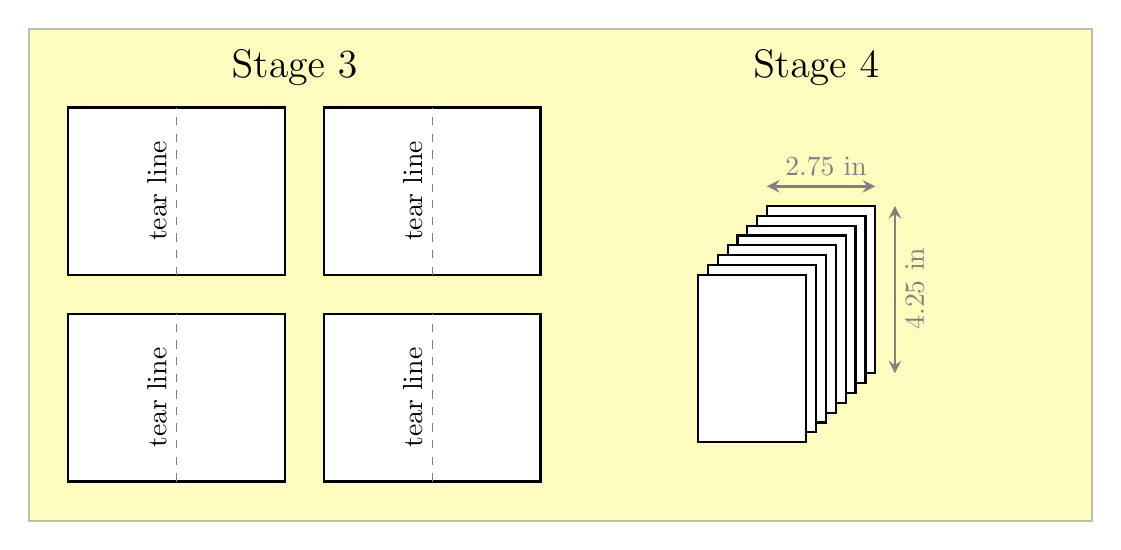
\begin{tikzpicture}[scale=0.5]
 \draw[black, thick, fill=yellow,opacity=0.25] (-1,-1) rectangle (26, 11.5);
 \draw[black, thick, fill=white] (0,0) rectangle (5.5, 4.25);
 \draw[black, thick, fill=white] (6.5,0) rectangle (12,4.25 );
  \draw[black, thick, fill=white] (0,5.25) rectangle (5.5, 9.5);
   \draw[black, thick, fill=white] (6.5,5.25) rectangle (12, 9.5);

  \draw[line width=0.5pt, dashed, gray](2.75,5.25)--(2.75,9.5);
\draw[line width=0.5pt, dashed, gray](2.75,0)--(2.75,4.25);
\draw[line width=0.5pt, dashed, gray](9.25,0)--(9.25,4.25);
\draw[line width=0.5pt, dashed, gray](9.25,5.25)--(9.25,9.5);
  
\node[rotate=90] at (2.25,2.13)   {tear line};
\node[rotate=90] at (2.25,7.38)   {tear line};
\node[rotate=90] at (8.75,2.13)   {tear line};
\node[rotate=90] at (8.75,7.38)   {tear line};

\draw[black, thick, fill=white] (17.75,2.75) rectangle (20.5, 7);
\draw[black, thick, fill=white] (17.5,2.5) rectangle (20.25, 6.75);
\draw[black, thick, fill=white] (17.25,2.25) rectangle (20, 6.5);
\draw[black, thick, fill=white] (17,2) rectangle (19.75, 6.25);
\draw[black, thick, fill=white] (16.75,1.75) rectangle (19.5, 6);
\draw[black, thick, fill=white] (16.5,1.5) rectangle (19.25, 5.75);
\draw[black, thick, fill=white] (16.25,1.25) rectangle (19, 5.5);
 \draw[black, thick, fill=white] (16,1) rectangle (18.75, 5.25);

 \draw[line width=1pt,gray, stealth-](17.75,7.5)--(19,7.5);
\draw[line width=1pt,gray, -stealth](19,7.5)--(20.5,7.5);
\node[gray] at (19.25,8)   {2.75 in};
\draw[line width=1pt,gray, stealth-](21,2.75)--(21,6);
\draw[line width=1pt,gray, -stealth](21, 6)--(21, 7);
\node[rotate=90, gray] at (21.5,4.9)   {4.25 in};

\node[] at (5.75,10.5)   {\Large{Stage 3}};
\node[] at (19,10.5)   {\Large{Stage 4}};
\end{tikzpicture}
\end{center}
At the end of the process you will have eight small rectangles, as shown in Stage 4.

\item Produce 104 units of product. 
\item Carefully measure the diagonal dimension and record it to the nearest .01cm.
\item Record your diagonal measurements in a spreadsheet of your choice.
\item Prepare a histogram of diagonal measures in the GeoGebra window below by copying and pasting your data column into the ``Student Data" column in GeoGebra.  Label all axis and display the upper and lower specification limits. 
\end{enumerate}

\begin{onlineOnly}
\begin{center} 
\geogebra{ajtk6jux}{950}{600} 
\end{center}
\end{onlineOnly}

% \begin{question}
%     Use the Pythagorean Theorem to complete the following expression for the length of the diagonal of the rectangle.  Then find the length of the diagonal to the nearest tenth of an inch.
%     $$2.75^2+\answer{4.25}^2=d^2$$
%     $$d=\answer{5.1}\,\text{in}$$
% \end{question}

% \begin{question}
%     You will be using centimeter rulers to measure the diagonals of the rectangles.  Let's convert the theoretical length of the diagonal to centimeters.  Use the 
%     \end{question}

Analysis/Discussion:

\begin{enumerate}
\item What is the advantage of drawing a picture of the data (histogram) compared to looking at a list of numbers?
\item Using only the list of measured values, what is your estimate of the average? Now using the histogram, what is your estimate of the average. Which method is easier to estimate the average? 
\item The histogram provides three pieces of information about the data. Comment on each of these as it relates to your data.
    \begin{enumerate}
\item The spread of the data compared to specification limits.  If the spread of the data is as wide as the specification limits, then the data is not very precise, and the process is likely to be making scrap. Scrap is when a measured value is outside the specification limits.
\item The position of the data compared to specification limits. If the histogram is well-centered within the specification limits, then the process is accurate. That is, the process is making product that is close to the nominal or midpoint of the specification range.
\item The pattern of the data. This is a crude, subjective assessment of the histogram but can be a useful indicator.  If the histogram is normally distributed, then the process is experiencing only common or natural causes of variation. If the histogram is not normally distributed, then the process is likely experiencing unwanted or assignable causes of variation.
    \end{enumerate}
\item What is the expected (calculated) value of the diagonal.
\item What is the percent error of the average of your data compared to the expected value?  

$$\text{Percent error} = \frac{|\text{Measured Value} – \text{Expected Value}|}{\text{Expected Value}} \times 100$$
\end{enumerate}
Do some research and discuss: 

Precision

Accuracy

Common or natural causes of variation

Assignable Cause of Variation    



\section*{Practice Problems}

\section*{References}
Wafer photo credit: \textit{Processed 200 mm Si Wafer} by Goldenvu CC BY-SA 4.0.

\end{document} 